\documentclass[a4paper,10pt]{book}
\usepackage[utf8x]{inputenc} 
\usepackage[french]{babel}
\usepackage[T1]{fontenc}
\usepackage{amssymb}
\usepackage[ampersand]{easylist}
\usepackage{amssymb}
\usepackage{tabu}
\renewcommand{\labelitemi}{$\bullet$}
%Options: Sonny, Lenny, Glenn, Conny, Rejne, Bjarne, Bjornstrup
 \renewcommand\labelitemii{$\square$}
\usepackage[Glenn]{fncychap}
\usepackage{amsfonts,amsmath,amssymb}
\usepackage{array,multirow,makecell}
\setcellgapes{1pt}
\makegapedcells
\usepackage{tabu}
\newcommand\tr{\rule{0pt}{4.5ex}}
\usepackage[table]{xcolor}
\usepackage{bbding}
\newcolumntype{R}[1]{>{\raggedleft\arraybackslash }b{#1}}
\newcolumntype{L}[1]{>{\raggedright\arraybackslash }b{#1}}
\newcolumntype{C}[1]{>{\centering\arraybackslash }b{#1}}
\usepackage{graphicx}
\usepackage{array,multirow,makecell}
\usepackage[ruled,vlined]{algorithm2e}
\usepackage{diagbox}
\usepackage{biblatex}
\usepackage{geometry}
\geometry{textwidth=15cm}
\usepackage{algorithmic}
\usepackage{layout}
\usepackage{french}
\addbibresource{sample.bib}
\usepackage[top=3cm, bottom=3cm, left=4.5cm, right=3cm]{geometry}
\usepackage{supertabular} % tableaux qui tiennent sur plusieurs 
\usepackage{fancyhdr}
\pagestyle{fancy}
\renewcommand{\headrulewidth}{1pt}
\fancyhead[L]{\leftmark}
\fancyhead[R]{}
\renewcommand{\footrulewidth}{1pt}
\renewcommand{\familydefault}{\rmdefault}
\fancyfoot[C]{\textbf{page \thepage}} 
\fancyfoot[L]{}
\fancyfoot[R]{}
\newcolumntype{C}{>{\centering\arraybackslash}X} 
\setcounter{secnumdepth}{4}
\setcounter{tocdepth}{4}
\begin{document}
\tableofcontents
\listoffigures

\newpage
\section*{Introduction G\'en\'erale} 
\par En Île-de-France le nombre des immeubles a augmenté de manière fréquente , 65\% \cite{einstein} de la population française vient en appartement en 2019 par rapport à 48\% en 2010​
La gestion d'immeubles devient très complexe et coûte plus d'argents et de temps.
Donc plusieurs acteurs intervient dans cette gestion.
De nos jours ,on a plus que le moitié de nombres des résidences sont des locataires comme en ile-de france 70\% des résidences sont des locataires  mais ils on a pas de moyen efficace pour communiquer , les échanges ne sont pas assez transparents pour tous ceux qui vivent et même pour les professionnels de immobilier . Selon les dernières estimations en date réelle  \cite{einstein} , le nombre de immeubles a augmenté de manière fréquente en Île-de-France au cours des douze derniers mois, 65\% de la population française vient en appartement en 2018 par rapport à 48\% en 2010.
Dans le même temps,5300 nouveaux appartements ont été mis en chantier, soit une augmentation de 12\% par rapport aux douze mois précédents.
 \begin{figure}[!h]
  \centering 
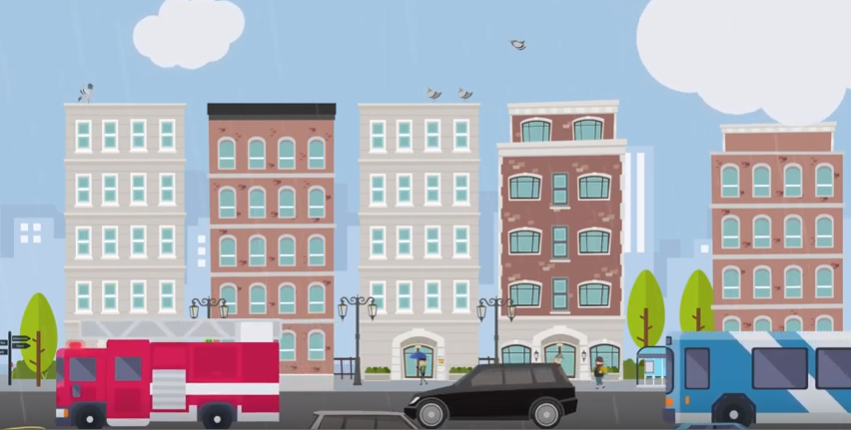
\includegraphics[width=0.9\textwidth]{imm.PNG}
\caption{Evolution du marché de l'immobilier}
\label{fig4}
\end{figure}

 Face aux problèmes de la gestion d'immeubles devient très complexe et coûte plus d'argents et de temps.
Donc plusieurs acteurs intervient dans cette gestion.

 \begin{figure}[!h]
  \centering 
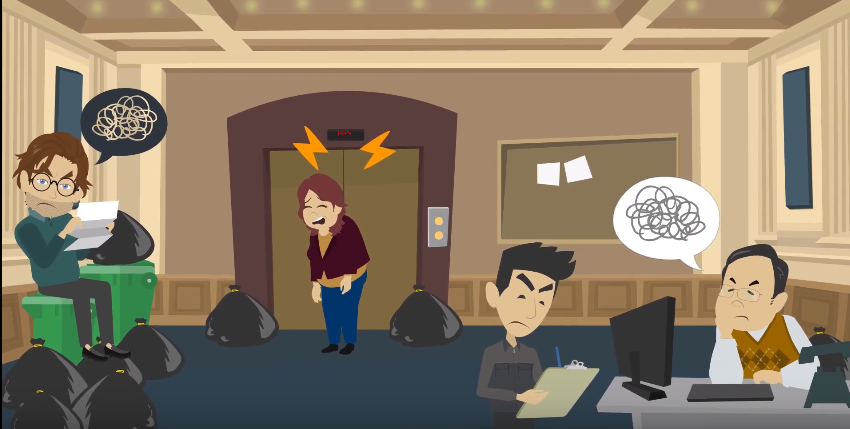
\includegraphics[width=0.9\textwidth]{problemeHL.PNG}
\caption{la gestion d'immeubles}
\label{fig4}
\end{figure}
\addcontentsline{toc}{chapter}{Introduction G\'en\'erale}
\renewcommand{\thesection}{\thechapter.\arabic{section}}
\chapter{Étude préalable et spécification des besoins}
\section*{Introduction} 
\addcontentsline{toc}{chapter}{Introduction}
\renewcommand{\thesection}{\thechapter.\arabic{section}}
\par  
Ce chapitre est une introduction de notre projet de stage professionnel. En effet ,ce projet nécessite une étude détaillée sur certaines notions qui touchent non seulement son cadre général , mais aussi sa réalisation. 
Nous commençons, d'abord par une présentation de l’entreprise d’accueil « Devagnos »,ensuite ,nous exposons, l’idée générale ,et  la problématique qui nous a poussée à réaliser ce projet. 
Par la suite , nous étudions les différentes méthodologies de développement et nous présentons une étude comparative afin de choisir la méthode que nous allons adopter par la réalisation. Enfin, nous mettrons en pratique la méthodologie sélectionnée pour notre application.

\section {Cadre de projet :}
    Cette première partie présente d’une manière générale  l’organisme d’accueil et l'idée maîtresse du projet.
  
\subsection{Présentation de l’entreprise d’accueil : }
\par La société  \textbf{Devagnos} \cite{dirac} est une société de développement spécialisée dans les solutions Web et les applications mobiles. Nous fournissons des solutions de pointe utilisant les dernières technologies de renommée mondiale.Fondée en 2015,et se présente comme une agence de communication numérique incontournable et une société de conseil en développement de logiciels nourrie par l'élite des développeurs talentueux de la région, ce qui lui permet d'offrir des packages complets de solutions aux clients. 
     
      \textbf{Devagnos} a développé un savoir-faire dans les « business applications » : les applications mobiles pour les entreprises. Les applications que nous développons pour le compte de nos clients sont conçues comme de véritables produits, dans une technologie native et garantissent la meilleure expérience utilisateur.
Ses fondateurs sont forts d’une expérience de plusieurs années dans la stratégie produit dans les logiciels, l’innovation technologique, le développement d’applications mobiles et les services aux entreprises dans l’informatique. 
Cette société est spécialisée en:


 \begin{itemize}
   \renewcommand{\labelitemi}{$\blacktriangleright$}
   \item Développement Web : les sites Web dynamiques, applications basées sur le Web, développement du contenu Web, optimisation des moteurs de recherche (SEO), développement d’eCommerce, etc.
    \item Développement Mobile : applications IOS, Android, Java, optimisation du site Web pour les navigateurs mobiles.
    \item 	Intégration Web
    \item 	Maintenance d'applications
         
   \end{itemize}
\newpage
\textbf{Coordonnées} 
\begin{itemize}
\item \textbf{Adresse:}  Avenue Combattant Supreme  Immeuble Ghomrassi 5ème Etage Monastir 5000
\item \textbf{Numéro Tel:} (+216) 54 173 773
\item \textbf{Site Web:} www.devagnos.com
 \end{itemize}
  \begin{figure}[!h]
  \centering 

\includegraphics[width=0.3\textwidth]{devagnoslogo.jpg}
\caption{Logo Devagnos}
\end{figure}
\subsection{Idée maîtresse du projet :} 
\par  Selon les dernières estimations en date réelle  \cite{einstein} , le nombre de immeubles a augmenté de manière fréquente en Île-de-France au cours des douze derniers mois, 65\% de la population française vient en appartement en 2018 par rapport à 48\% en 2010.
​Dans le même temps,5300 nouveaux appartements ont été mis en chantier, soit une augmentation de 12\% par rapport aux douze mois précédents.



\par  Face aux problèmes de la gestion d'immeubles devient très complexe et coûte plus d'argents et de temps.
Donc plusieurs acteurs intervient dans cette gestion.

\section {Problématique : }
\par  De nos jours ,on a plus que le moitié de nombres des résidences sont des locataires mais ils on a pas de moyen efficace pour communiquer , les échanges ne sont pas assez transparents pour tous ceux qui vivent et même pour les professionnels de immobilier .

\par La communication entre les résidents , leurs prestataires et les collaborateurs est a toujours avec une trace écrite,qui établir une trace sur papier aide à conserver les informations importantes dans la tête des collaborateurs ou une écoute active pour informer les résidents .


\section{Étude de l’existant : }
\par
    La résidence est basée sur les affiches papiers dans les halls. Elle est encore traditionnelle, où les relations entre les différents acteurs sont encore fragiles. L’identification et la localisation des lots ne sont pas encore évidentes et la gestion est décentralisée. 

    Le résultat est une communication non optimisée  et une perte importante de temps et de coût. 

\section{Critique de l’existant :}
Tout le monde connaît le tableau d'affichage des immeubles, situé en principe dans l'entrée des résidences, il permet de communiquer par notes avec les résidents, mais qu'en est-il de son efficacité et surtout à l'heure d'internet.
 Le tableau d'affichage a une dimension qui n'est pas extensible, afficher tous les documents nécessaires peut être difficile, voir impossible, il est donc nécessaire que toutes les notes soient directement visibles. 
 


  \begin{figure}[!h]
  \centering 
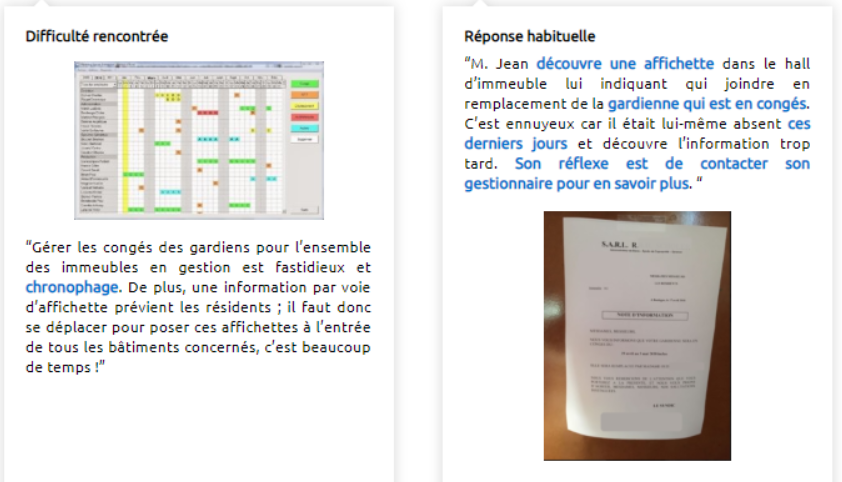
\includegraphics[width=0.9\textwidth]{avis.png}
\caption{ Avis d’un résident}
\label{fig4}
\end{figure}
La figure 1.2 montre quelques avis des résidents \cite{einstein} :
On a trouvé les problèmes d'adresses emails qui changent ( déménagements, changement d'email, démission du conseil syndical...) en s'adressant directement à l'immeuble​
\section{Solution proposée : <<HOMELINKS>>}
 Les gestionnaires peuvent diffuser la publication des affiches par voie digitale pour l’ensemble des immeubles d’un seul clic. 

    Ils peuvent aussi programmer leur envoi. Les destinataires sont alors prévenus sans pour autant devoir lire un papier dans le hall et ainsi peuvent prendre leurs dispositions par avance. 

     De plus, le calendrier classe toutes les informations faciles à retrouver .  
   \\\
\par \textbf{Simplifier les relations }
     Pour en finir avec les incompréhensions ou les informations partielles,Homelinks vous permet de trier, ordonner et classer vos communications pour une usage devenu facile. 
\\
 \par \textbf{Animer le réseau }
     Homelinks \cite{hl} offre une gamme de services pour libérer le potentiel d’un groupe en gardant le contact avec les relais locaux et favorisant  une pleine participation. 
\\
 \par \textbf{Faciliter les échangés }
    Que ce soit pour une urgence, une actualité ou une consultation,Homelinks ouvre la résidence sur plus de transparence et de réactivité sur l’ensemble des sujets.\\\
    
     Aussi HOMELINKS offre une solution numérique simple et utile autour de deux axes : \\
– la communication et la gestion optimisées de l’immeuble. \\
– la mise en connexion de l’immeuble avec son environnement immédiat​

\section{Spécification des besoins  }
\subsection{ Besoins fonctionnels }
\par 
Les besoins fonctionnels représentent les attentes de chaque acteur de l’application à développer. Toute solution conceptuelle doit satisfaire, préalablement, à des besoins fonctionnels afin de délimiter le périmètre fonctionnel de l’application et surveiller la traçabilité des besoins lors de la phase de développement. Pour notre application, ses besoins fonctionnels de bases sont :
\\
\par\textbf{Inscription :} Le système doit permettre aux utilisateurs de pouvoir s’inscrire de façon autonome via l’application.
\par\textbf{Authentification :} Pour pouvoir bénéficier les services offertes par l’application, il est nécessaire de s’authentifier et accéder à son compte personnel grâce à un pseudo et un mot de passe.

\par\textbf{Publier un message :} Les utilisateurs peuvent déclarer un évènement et le suivre, promouvoir les informations liées à l’immeuble, répondre à des consultations, connaitre tous les occupants et intervenants de l’immeuble, le tout dans un environnement dédié et sécurisé.
\par\textbf{Consulter le calendrier d'évènements:} L’utilisateur peut consulter des évènements dans le calendrier et les évènements prévues quotidiennement, agenda du jour, agenda sur 3 jours, agenda hebdomadaire ou calendrier du mois.

\par\textbf{Gestion : }  L’administrateur peut ajouter, modifier ou  supprimer une ou plusieurs utilisateurs ou immeubles.  Il peut également consulter le statistique de création d'immeubles et d'utilisateurs et la liste d'historique .
\subsection{ Besoins non fonctionnels }

\par 
Les besoins non fonctionnels décrivent toutes contraintes auxquelles soumis le système pour l’amélioration de son bon fonctionnement. Parmi ces besoins, on cite :
\\
\par\textbf{La rapidité de traitement :} En effet, vu le nombre important des transactions quotidiennes, il est impérativement nécessaire que la durée d'exécution des traitements s'approche le plus possible du temps réel.
\par\textbf{La mobilité :} Une aplication Web toujours disponible quand  nécessaire  
\par\textbf{Maintenabilité :} le code de l’application doit être bien compréhensible et bien clair pour l’observateur  pour permettre des futures évolutions ou améliorations.

\par\textbf{Sécurité :} toute personne qui doit utiliser l’application doit s’authentifier.

\par\textbf{Efficacité :} le système doit fournir les bons résultats qui répondent exactement aux besoins de l’application.
\par\textbf{La convivialité :} Le futur logiciel doit être facile à utiliser. En effet, les interfaces utilisateurs doivent être conviviales c'est-à-dire simples, ergonomiques et adaptées à l'utilisateur.

\par\textbf{La confidentialité:} Homelinks met en priorité la protection des données personnelles de ses utilisateurs. La divulgation de l’identité des membres Homelinks, ainsi que toutes informations personnelles les concernant est strictement interdite sans avoir, au préalable, reçu une autorisation écrite de leur part. 

\section{Conclusion}
\par   Dans ce chapitre, nous avons présenté une étude de l’existant, la problématique et la solution proposée pour la gestion de projet. Dans le chapitre suivant, nous présenterons la phase d’analyse et de conception de notre application en utilisant la méthodologie UML. 

\chapter{ Étude conceptuelle de l’application }
\section{Introduction}
\par
  Afin de mener à bien le développement de module de Homelinks ,nous allons procéder à une étude conceptuelle de l’application suivant une démarche modulaire. Pour se faire, nous choisissons le langage de modélisation UML comme méthode de conception. L’UML (Unified Modeling Language) est une notation semi formelle.  
  \\
      Il part de la réponse au cahier de charge jusqu’à la rédaction du document de la conception. Il couvre toutes les phases d'un projet. Cette notation offre une analyse permettant une formalisation du système à développer en réponse à l’expression des besoins par les utilisateurs.  
      \\\
       L’analyse se concrétise par l’élaboration de tous les diagrammes donnant une représentation du système tant statique (diagramme de classe principalement), que dynamique (diagramme de séquence, état-transition…). 
\section{Spécification semi-formelle des besnoins } 
\par Pour une spécification semi-formelle des besoins, la sémantique sera clairement spécifiée et décrite. Ainsi, on a été intéressé à spécifier les acteurs de nos diagrammes concernant la conception.
 \subsection{Les acteurs } 
\par Nous allons maintenant énumérer les acteurs susceptibles d'interagir avec le système. Tout d'abord, nous commençons par définir ce qui est un acteur. 
\par \textbf{Définition :} un acteur représente l'abstraction d'un rôle joué par des entités externes (utilisateur, dispositif matériel ou autre système) qui interagissent directement avec le système étudié. 
\par  
   Les acteurs sont définis comme étant les utilisateurs directs de l’application. On distingue à ce propos trois acteurs principaux: 
\vspace{3cm}
\begin{figure}[!h]
\centering 
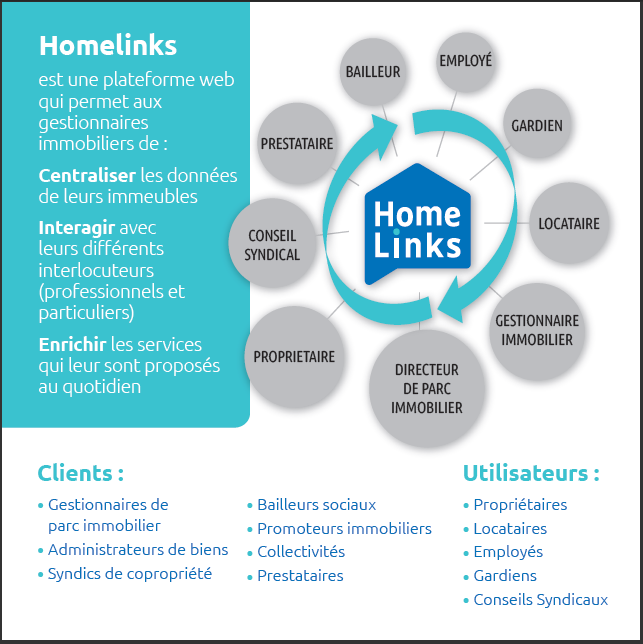
\includegraphics[width=0.8\textwidth]{acteurs.png}
\caption{Présentation de «Homelinks» \cite{hl}}
\end{figure}
\vspace{3cm}

\subsection{Diagrammes des cas d'utilisation }
\par\textbf{Définition :} Les diagrammes de cas d'utilisation sont des diagrammes UML utilisés pour donner une vision globale du comportement fonctionnel d'un système logiciel. Ils sont utiles pour des présentations auprès de la direction ou des acteurs d'un projet, mais pour le développement, les cas d'utilisation sont plus appropriés. Un cas d'utilisation représente une unité discrète d'interaction entre un utilisateur (humain ou machine) et un système. Il est une unité significative de travail. Dans un diagramme de cas d'utilisation, les utilisateurs sont appelés acteurs (actors), ils interagissent avec les cas d'utilisation (use cases). 

\subsubsection{Diagramme de cas d'utilisation globale }
\par La figure suivante illustre le diagramme de cas d’utilisation global présente les différents besoins fonctionnels nécessaires à l’élaboration de notre projet, ce diagramme englobe les cas d’utilisation suivants : \\
\par Gérer les utlisateurs et les immeubles par l’administrateur
 et permet à tout Utilisateur de la Plateforme de publier un message, dont le contenu est sous un format textuel,photo ou lien internet ou tout autre format permettant le transfert d’information. Ce Post peut être destiné à certains ou à l’ensemble des Utilisateurs d’un même immeuble.Les Posts sont affichés dans le fil d’actualité des Utilisateurs concernés. Mais avant toute interaction avec le système l’utilisateur doit s’authentifier.
\vspace{3cm}
\begin{figure}[!h]
\centering 
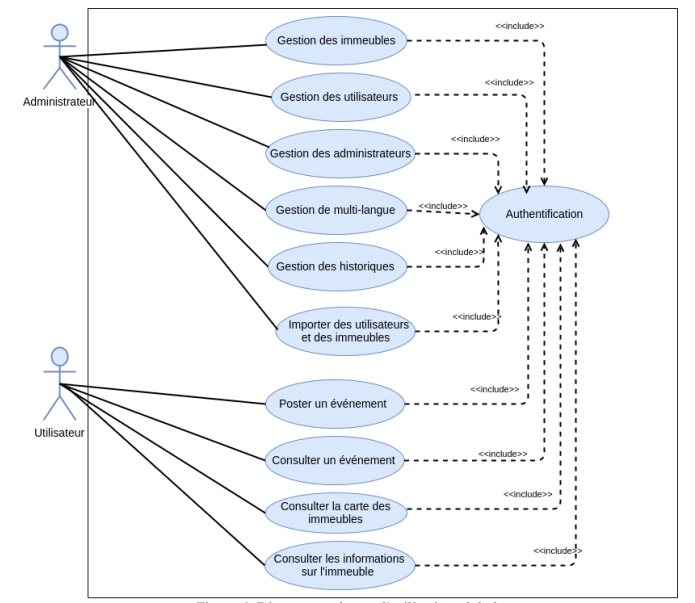
\includegraphics[width=1\textwidth]{usecase.png}
\caption{Diagramme de cas d’utilisation Global }
\label{fig4 }
\end{figure}

\subsection{Diagramme de classes  } 

\par Le diagramme de classes identifie la structure des classes d’un système, y compris les
propriétés et les méthodes de chaque classe. Les diverses relations, telles que la relation
d’héritage par exemple, qui peuvent exister entre les classes sont également représentées.
Le diagramme de classes est le diagramme le plus largement répandu dans les spécifications
d’UML.
\vspace{3cm}
\begin{figure}[!h]
\centering 
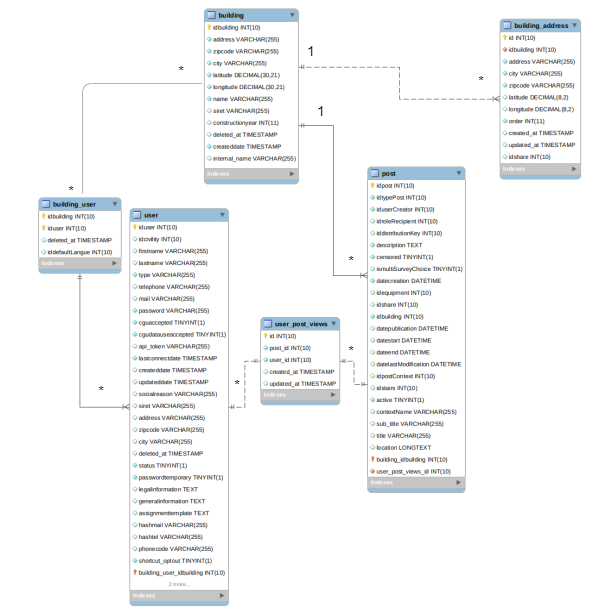
\includegraphics[width=1\textwidth]{clss.png}
\caption{Diagramme de cas d’utilisation Global }
\label{fig4 }
\end{figure}


\vspace{3cm}

\section{Conclusion}
\par 
   Dans ce chapitre, nous avons décrit la conception suivant la démarche UML. 
   Cette conception nous permet d’entamer la réalisation et l’implémentation del’application de gestion des comptes rendus. 

 
\chapter{Développement et réalisation }
\par
\section{Introduction}
\par  
   Ce chapitre a pour objectif de présenter le produit. C’est la phase de réalisation de cette application qui utilise des technologies spécifiques. Ce chapitre est composé de deux parties : on présente en premier lieu une description de l’environnement de travail, à savoir l’environnement logiciel et l’environnement matériel ainsi que nos choix techniques adoptés pour la réalisation de cette application.  
\\
   En second lieu, nous présentons les logiciels utilisés lors de la conception et le développement de ce système. Enfin, nous terminons par présenter des maquettes de capture d’écrans relative à l’application. 

\section{Environnements logiciels}

Cette partie est consacrée à la présentation des différentes outils logiciels utilisés pour le développement de notre application

\subsection{  Angular}
est un Framework côté client \cite{angular} open source basé sur TypeScript dirigée par l'équipe du projet Angular à Google et par une communauté de particuliers et de sociétés. On a utilisé ce Framework pour le développement frontend de l’application.
\begin{figure}[!h]
\centering 

\includegraphics[width=0.4\textwidth]{d.png}
\caption{Logo Angular }
\end{figure}

\subsection{ Visual Studio Code }
 Visual Studio Code : est un éditeur de code open-source \cite{vsc}, gratuit et multiplateforme (Windows, Mac et Linux), développé par Microsoft. Principalement conçu pour le développement d'application avec JavaScript, TypeScript et Node.js, l'éditeur peut s'adapter à d'autres types de langages grâce à un système d'extension bien fourni. 
\begin{figure}[!h]
\centering 

\includegraphics[width=0.4\textwidth]{vsc.png}
\caption{Logo Visual Studio Code }
\end{figure}
\subsection{MySQL Workbench }
   MySQL Workbench: est un outil visuel unifié pour les architectes de bases de données \cite{wb}, les développeurs et les administrateurs de base de données.MySQL Workbench fournit la modélisation des données, le développement SQL et des outils d'administration complets pour la configuration du serveur, l'administration des utilisateurs, la sauvegarde et bien plus encore.

     MySQL Workbench est disponible sur Windows, Linux et Mac OS X. 
 \begin{figure}[!h]
\centering 

\includegraphics[width=0.4\textwidth]{raw.png}
\caption{Logo MySQL Workbench }
\end{figure}
\subsection{Laravel }
          Laravel : est un Framework web open-source écrit en PHP respectant le principe modèle-vue-contrôleur et entièrement développé en programmation orientée objet \cite{laravel}. On a utilisé ce Framework pour le développement backend de l’application. 
          
          
 \begin{figure}[!h]
\centering 

\includegraphics[width=0.4\textwidth]{LaravelLogo.png}
\caption{Logo Laravel }
\end{figure}

\subsection{Latex (Overleaf) }
LATEX est un langage et un système de composition de documents créé par Leslie Lamport \cite{latex} . Il s'agit d'une collection de macro-commandes destinées à faciliter l'utilisation du « processeur de texte » TeX.
\begin{figure}[!h]
\centering 

\includegraphics[width=0.4\textwidth]{latex.png}
\caption{Logo Overleaf }
\end{figure}
\subsection{Draw.io}
Draw.io (anciennement Diagramly) est un logiciel libre de diagramme en ligne. Vous pouvez l'utiliser comme un fabricant d'organigramme \cite{drawio}, logiciel de diagramme de réseau, de créer UML en ligne, comme un outil de diagramme ER, pour concevoir le schéma de base de données, pour construire BPMN en ligne, sous forme de diagramme fabricant de circuit, et plus encore. Il est ciblé comme une fonctionnalité de 90\% en ligne alternatif Visio et inclut le format Visio import.
\begin{figure}[!h]
\centering 

\includegraphics[width=0.4\textwidth]{drawio.png}
\caption{Logo Draw.io }
\end{figure}

\section{Choix techniques }
\subsection{ Architecture de l’application}
\par
      L’application de gestion des projets est une application qui se connecte à un serveur de base de données via Internet \cite{3tiers}, afin de récupérer les données, ce qui nécessite l’intégration d’un serveur web entre l’application client et le serveur de bases des données. C’est pour cela que nous avons suivi l’architecture 3-tiers pour notre application client-serveur. 
      
\vspace{3cm}
\begin{figure}[!h]
\centering 

\includegraphics[width=0.6\textwidth]{3-tier_architecture-2.png}
\caption{Logo  Architecture 3-tiers  }
\end{figure}

\vspace{1cm}
\subsection{Architecture Modèle/Vue/Contrôleur }
\par   Le modèle MVC (modèle, vue et contrôleur) est un concept très puissant qui intervient dans la réalisation d’une application \cite{mvc}. Son principal intérêt est la séparation des données (modèle), de l’affichage (vue) et des actions (contrôleur)
      \begin{figure}[!h]
\centering 
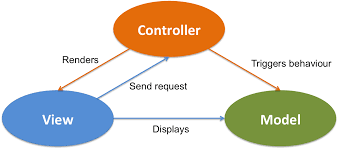
\includegraphics[width=0.6\textwidth]{mvc.png}
\caption{Logo MVC }
\end{figure}


\section{Présentation des interfaces de l’application }
\par \par Dans la partie qui va suivre, nous allons donner un aperçu des interfaces de l’application
web développées illustrant les différents cas d’utilisation déjà vus dans le chapitre président.


\subsection{Interface d'authentification}
L'authentification est l'interface qui s'affiche en premier, Chaque personne doit insérer son pseudo	 et son mot de passe. Dans le cas où la combinaison n'est pas valide un message d’erreur sera affiché.
\begin{figure}[!h]
\centering 
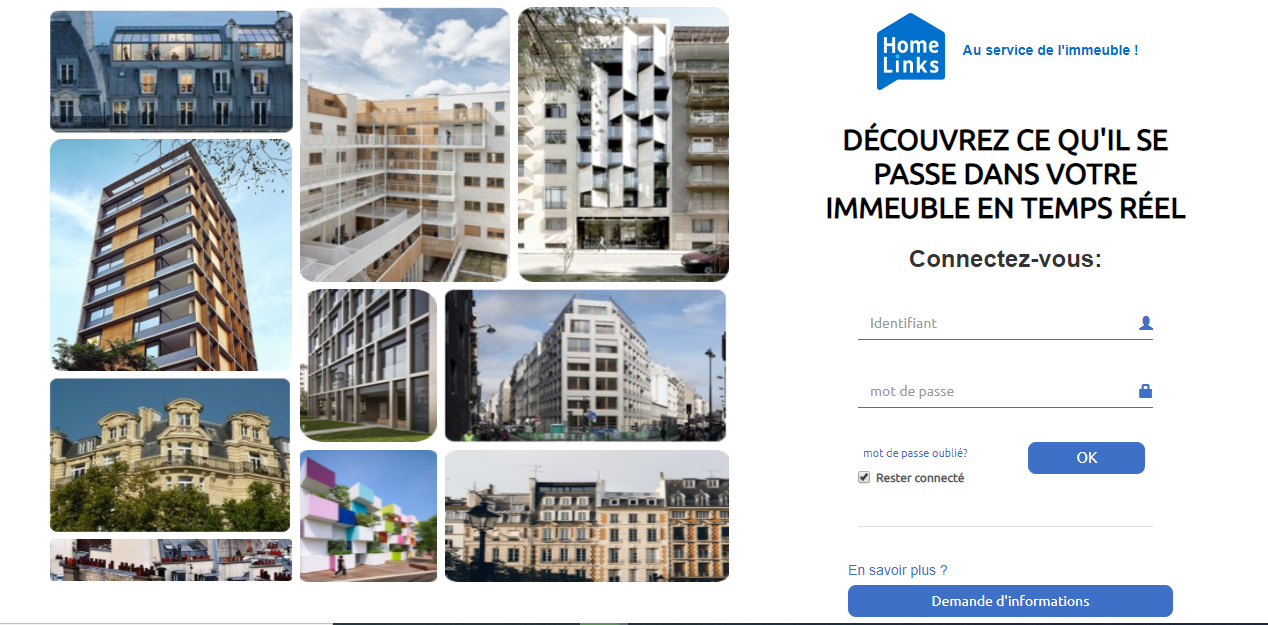
\includegraphics[width=1\textwidth]{auth.PNG}
\caption{Interface d'authentification}
\end{figure}
\subsection{Interface de Dashbord}
   Dans le cas où la connexion aurait été établie par l’administrateur , il va voir comme première interface le Dashboard qui lui propose un certain nombre des fonctionnalités comme ça sera présenté dans les deux figures ci-dessous 
\begin{figure}[!h]
\centering 
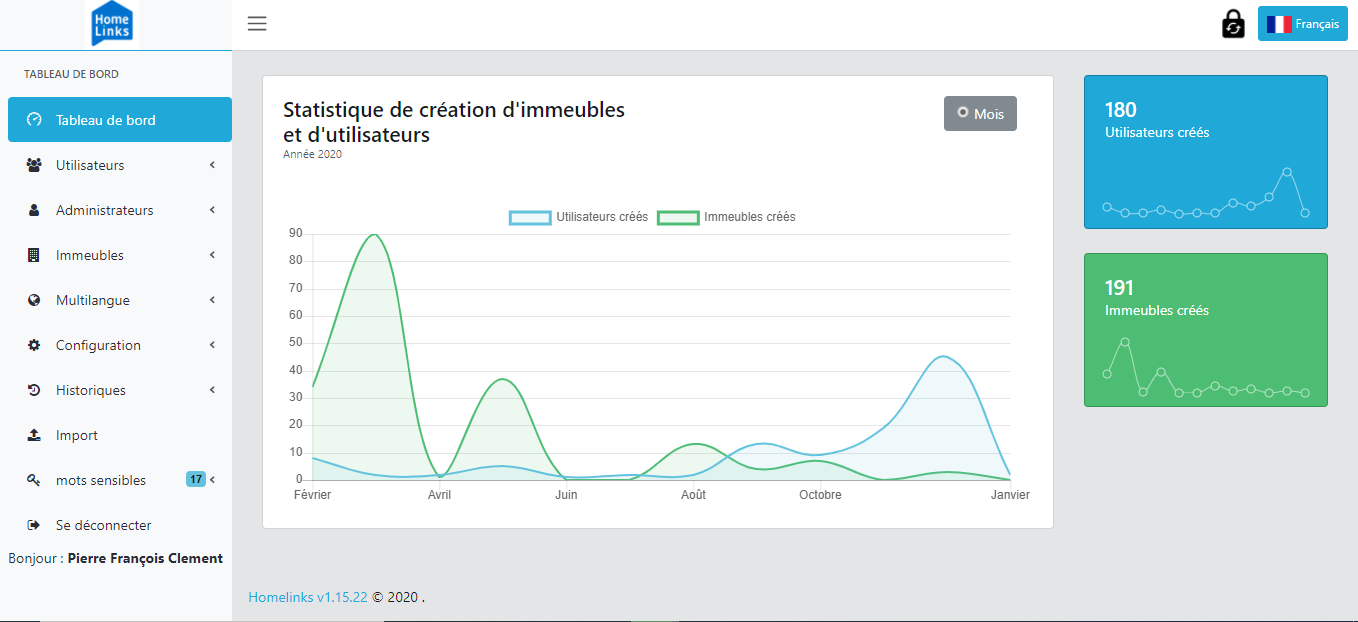
\includegraphics[width=1\textwidth]{dashbord.PNG}
\caption{Interface de Dashbord}
\end{figure}
L’administrateur peut distinguer facilement entre le nombre de créations d’immeuble et d’utilisateurs.  

\subsection{Interface de l'importation}
Pour créer des nouveaux utilisateurs, des administrateurs ou des immeubles facilement et rapidement on a mis en haut à droite de l'interface une liste des choix. 

\begin{figure}[!h]
\centering 
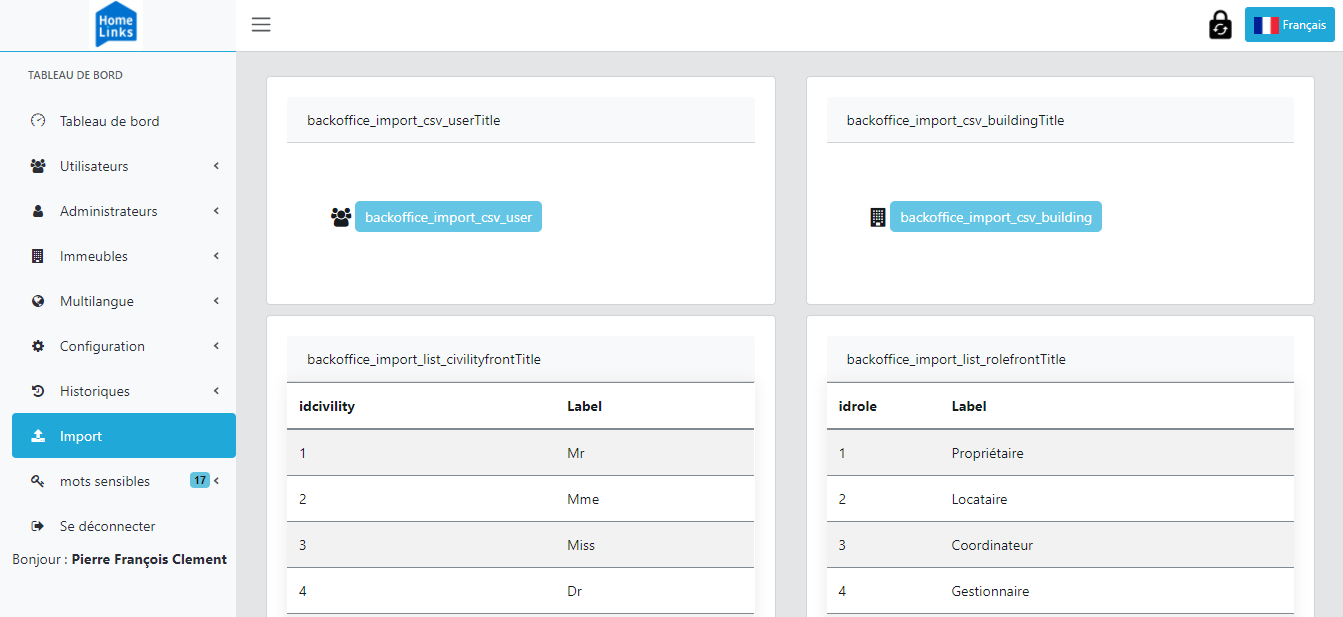
\includegraphics[width=1\textwidth]{import.PNG}
\caption{Interface d'importation}
\end{figure}
\vspace{4cm}
 L’importation des données, qui sont soit des utilisateurs soit des immeubles (un fichier sous forme  Excel, csv… ), peut se faire en simple clique sur le module d’import dans la liste de choix qui se trouve à gauche «tableau de bord»
 
\subsubsection{ Cas d’importation «Utilisateur»: }
 En cliquant sur le bouton «import Utilisateur» , une interface s’affiche avec le nombre des utilisateurs leurs rôles et leurs titres. 

Une importation réussie signifie l’ajout  d’un ou plusieurs nouveaux utilisateurs dans la base de données .
      

 \subsubsection{ Cas d’importation «Immeuble»: }
L’administrateur peut ajouter une nouvelle immeuble en cliquant sur un simple bouton «import immeuble».

\begin{figure}[!h]
\centering 
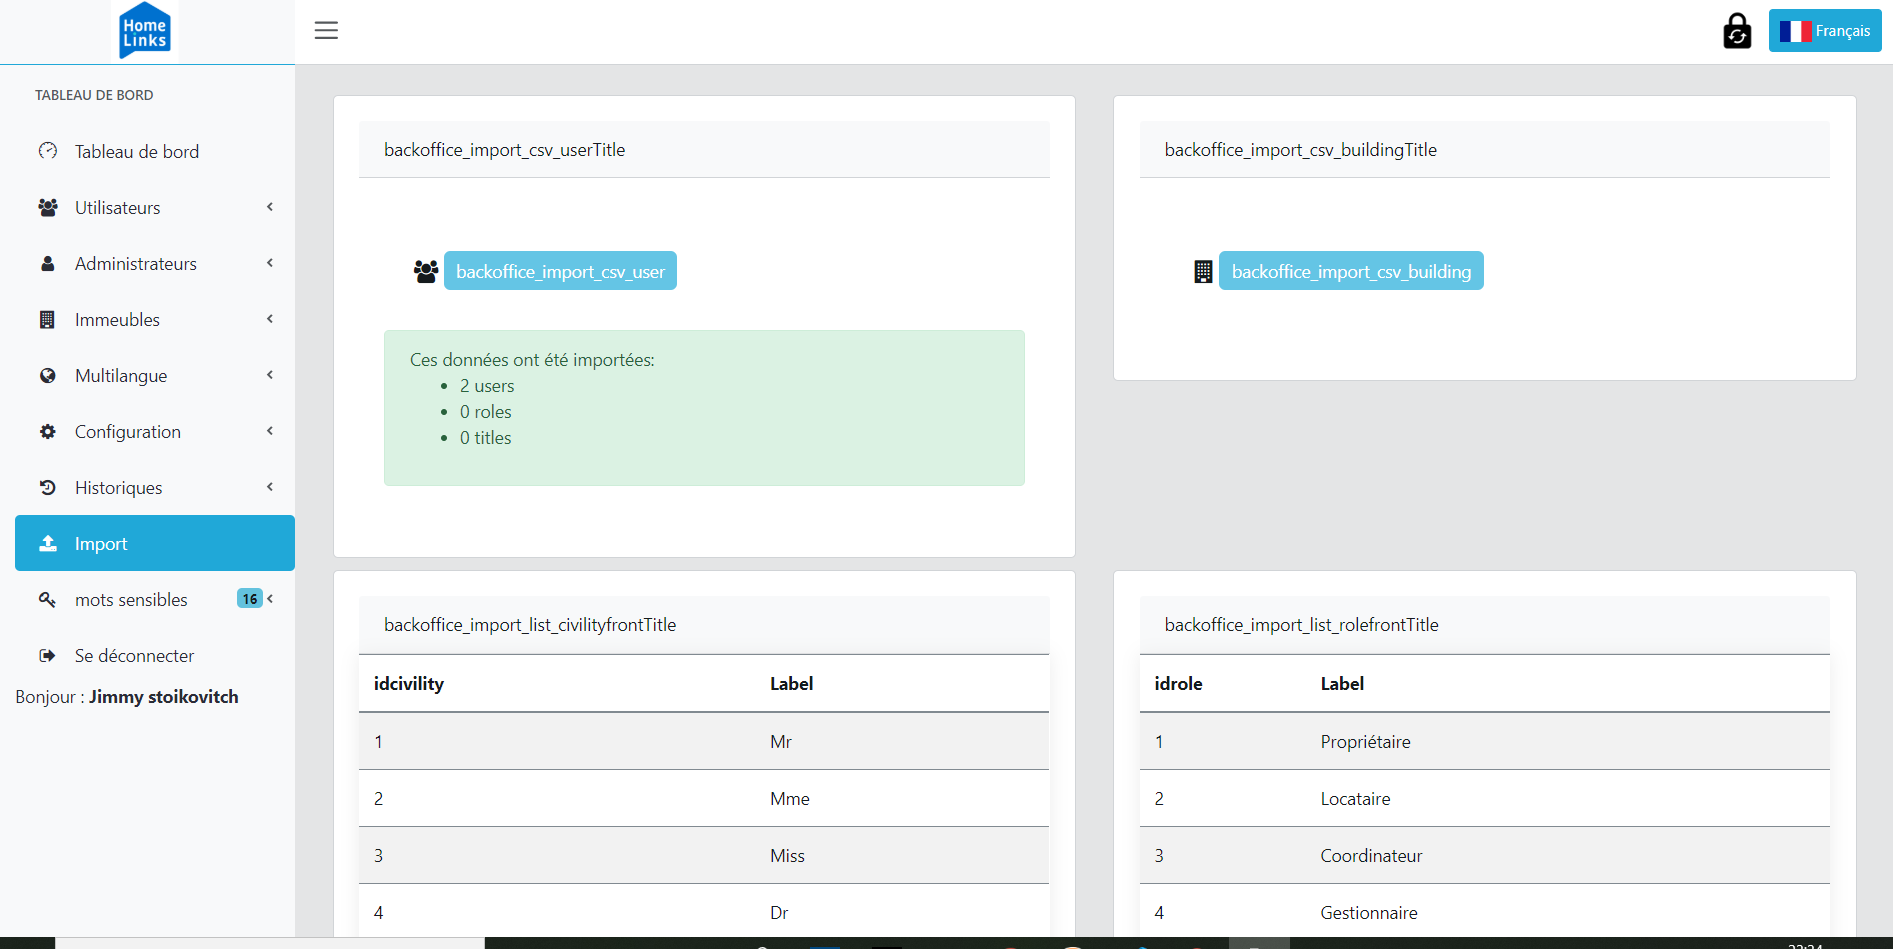
\includegraphics[width=1\textwidth]{imp.png}
\caption{Interface  d’importation des utilisateurs}
\end{figure}
\subsection{Interface de carte des immeubles   }
\par 

 
\textbf{Centrer la carte sur le groupe immeuble  }
En se connectant avec son propre login et en cliquant sur immeuble dans la carte géographique, toutes les immeubles aux quelles appartient l’utilisateur correspondant s’affichent avec ses centres d’intérêt .
\vspace{1cm}
\begin{figure}[!h]
\centering 
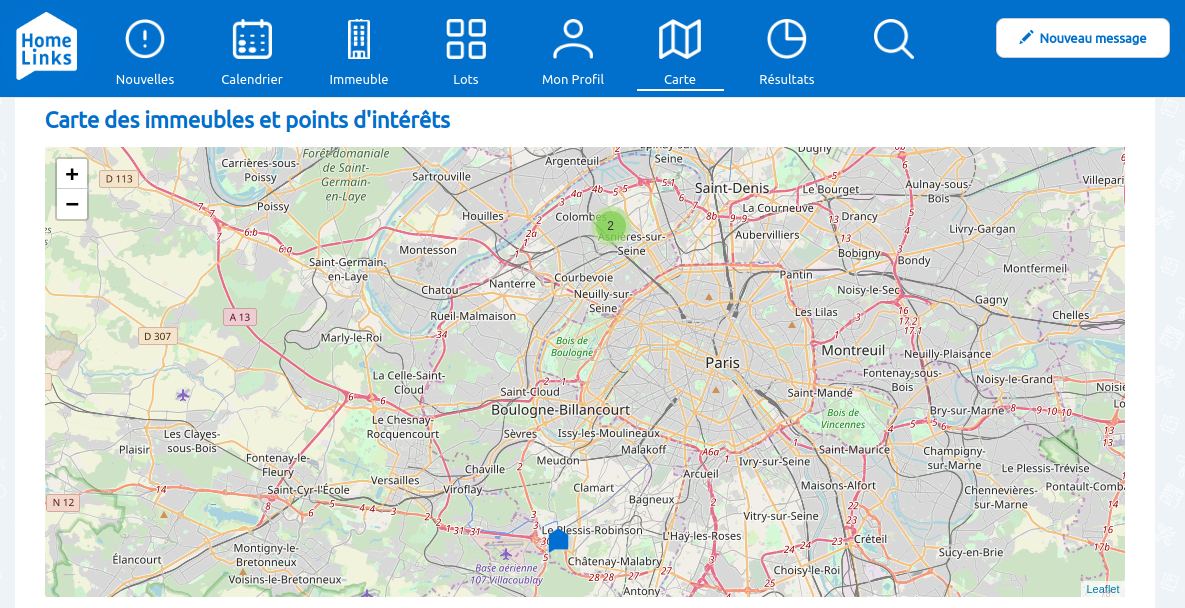
\includegraphics[width=1\textwidth]{carte.png}
\caption{Interface de carte des immeubles }
\end{figure}

 Pour faciliter la recherche d’immeuble pour l’utilisateur et en répondant aux besoins de client , nous avons ajouté deux adresses supplémentaires pour chaque immeuble .

\newpage
\section*{ Conclusion générale et perspectives }
Au cours de ce projet de stage professionnel on a conçu et implémenté un module dans une plateforme ayant pour objectif de répondre aux besoins des clients et ses attentes selon le cahier des charges signé a l’avant. \\
 Ce travail nous a permis d’utiliser en pratique nos connaissances acquises. C’était aussi une bonne opportunité  pour se familiariser avec l’environnement de travail au sein de la société Devagnos. 
\\
    Nous avons franchi et décrit toutes les étapes nécessaires pour la réalisation du travail, de la contribution à la réalisation du cahier des charges, à l’étude de l’existant, de l’analyse, aux spécifications et à la conception, pour finir avec la réalisation. \\
      La conception  avec le formalisme UML nous a permis de bien modéliser notre système de manière à ce que la compréhension de celui-ci devient plus facile et que le développement soit plus rapide.  \\
          L’utilisation des technologies bien choisies dans le développement web  nous a facilité la réalisation et a permis de gagner au niveau du temps et de la rentabilité. Pour conclure, la réalisation de ce projet nous a été très bénéfique dans notre formation, dans la mesure où il nous a aidé à mettre en œuvre nos acquis théoriques et pratiques reçus tout au long de notre formation à l’école pluridisciplinaire internationale de Sousse et surtout à les confronter avec les exigences de la société.  \\
          Il a été aussi une occasion pour s’intégrer à la vie professionnelle et pour confronter des technologies très répandues dans le développement web. 

\medskip
 
\printbibliography
\end{document}